% !TEX root = ../../main.tex
% File: part2/chapters2/chap2_1.tex

\section{Thiết lập Môi trường với Hệ sinh thái Hugging Face}
\label{sec:hf_ecosystem}

\begin{center}
    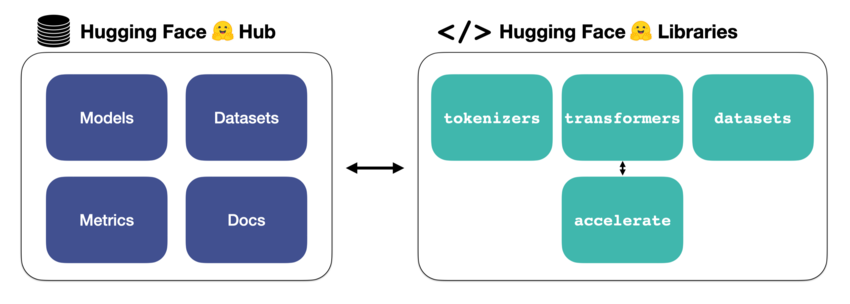
\includegraphics[width=0.8\textwidth]{hf_ecosystem_logos.png}
    \captionof{figure}{Các thư viện cốt lõi trong Hệ sinh thái Hugging Face.}
    \label{fig:hf_ecosystem_logos}
\end{center}

Hugging Face đã phát triển từ một công ty chatbot thành trung tâm của cộng đồng NLP mã nguồn mở. Hệ sinh thái của họ cung cấp các công cụ mạnh mẽ, được thiết kế để hoạt động liền mạch với nhau, giúp đơn giản hóa và chuẩn hóa quy trình làm việc với các mô hình Transformer.

Để bắt đầu, chúng ta cần cài đặt và hiểu vai trò của bốn thư viện cốt lõi.

\begin{minted}{bash}
# Cài đặt các thư viện chính bằng pip
pip install transformers datasets accelerate evaluate
\end{minted}

Hãy cùng tìm hiểu vai trò của từng thư viện.

\subsection{Transformers: Trái tim của Hệ sinh thái}
\label{ssec:hf_transformers}
\begin{itemize}
    \item \textbf{Mục đích:} Cung cấp một giao diện đơn giản và nhất quán để tải về, sử dụng và huấn luyện hàng nghìn mô hình Transformer đã được huấn luyện trước (pre-trained models) từ \textbf{Hugging Face Hub}.
    \item \textbf{Hugging Face Hub là gì?} Là một nền tảng trực tuyến (tương tự như GitHub) nơi cộng đồng có thể chia sẻ và khám phá các mô hình, bộ dữ liệu và các bản demo. Đây là tài nguyên quan trọng nhất trong hệ sinh thái.
    \item \textbf{Các thành phần chính:}
        \begin{itemize}
            \item \textbf{`pipeline`:} Một API cấp cao, cực kỳ dễ sử dụng để thực hiện các tác vụ NLP phổ biến chỉ trong vài dòng code. Rất tuyệt vời cho việc thử nghiệm nhanh và tạo demo.
            \item \textbf{`AutoModel`, `AutoTokenizer`:} Các lớp "tự động" thông minh. Bạn chỉ cần cung cấp tên của một mô hình trên Hub (ví dụ: `"bert-base-uncased"`), các lớp này sẽ tự động tìm, tải về và khởi tạo đúng kiến trúc mô hình và tokenizer tương ứng.
            \item \textbf{`Trainer` API:} Một API huấn luyện cấp cao, mạnh mẽ, giúp xử lý tất cả các công việc phức tạp của vòng lặp huấn luyện (training loop) như tối ưu hóa, lên lịch tốc độ học (learning rate scheduling), đánh giá, và lưu trữ mô hình.
        \end{itemize}
\end{itemize}

\begin{example}{Sử dụng `pipeline` để phân loại cảm xúc}{ex:hf_pipeline}
    \begin{minted}{python}
    from transformers import pipeline

    # Tải một mô hình đã được fine-tune cho phân tích cảm xúc
    # Lần đầu chạy, pipeline sẽ tự động tải mô hình từ Hub
    classifier = pipeline("sentiment-analysis")

    # Sử dụng mô hình
    result = classifier("Hugging Face is democratizing NLP!")
    print(result)
    # Output: [{'label': 'POSITIVE', 'score': 0.9998...}]
    \end{minted}
\end{example}

\subsection{Datasets: Quản lý Dữ liệu Hiệu quả}
\label{ssec:hf_datasets}
\begin{itemize}
    \item \textbf{Mục đích:} Cung cấp một cách thức hiệu quả và tiêu chuẩn hóa để tải về, xử lý, và làm việc với các bộ dữ liệu, đặc biệt là các bộ dữ liệu lớn.
    \item \textbf{Các tính năng chính:}
        \begin{itemize}
            \item \textbf{Truy cập hàng nghìn bộ dữ liệu:} Tương tự như `transformers`, thư viện `datasets` cho phép bạn tải về hàng nghìn bộ dữ liệu công khai từ Hugging Face Hub chỉ bằng một dòng lệnh (`load\_dataset`).
            \item \textbf{Xử lý hiệu quả bộ nhớ (Memory-mapping):} Đối với các bộ dữ liệu khổng lồ (hàng trăm GB), `datasets` không tải toàn bộ vào RAM. Thay vào đó, nó sử dụng kỹ thuật memory-mapping (được hỗ trợ bởi Apache Arrow), cho phép bạn truy cập và xử lý dữ liệu ngay trên đĩa cứng một cách cực kỳ nhanh chóng.
            \item \textbf{API xử lý mạnh mẽ:} Cung cấp các phương thức như `.map()`, `.filter()`, `.shuffle()` cho phép bạn áp dụng các hàm tiền xử lý (như tokenization) lên toàn bộ bộ dữ liệu một cách song song và hiệu quả.
        \end{itemize}
\end{itemize}

\begin{example}{Tải và xử lý một bộ dữ liệu với `datasets`}{ex:hf_datasets}
    \begin{minted}{python}
    from datasets import load_dataset
    from transformers import AutoTokenizer

    # Tải bộ dữ liệu GLUE, tác vụ MRPC
    raw_datasets = load_dataset("glue", "mrpc")
    # >>> raw_datasets
    # DatasetDict({
    #     train: Dataset({
    #         features: ['sentence1', 'sentence2', 'label', 'idx'],
    #         num_rows: 3668
    #     })
    #     ...
    # })

    # Tải tokenizer tương ứng với một checkpoint
    checkpoint = "bert-base-uncased"
    tokenizer = AutoTokenizer.from_pretrained(checkpoint)

    # Viết một hàm để tokenize dữ liệu
    def tokenize_function(example):
        return tokenizer(example["sentence1"], example["sentence2"], truncation=True)

    # Áp dụng hàm này lên toàn bộ bộ dữ liệu
    # batched=True xử lý nhiều mẫu cùng lúc để tăng tốc
    tokenized_datasets = raw_datasets.map(tokenize_function, batched=True)
    print(tokenized_datasets)
    \end{minted}
\end{example}

\subsection{Accelerate: Đơn giản hóa Huấn luyện Phân tán}
\label{ssec:hf_accelerate}
\begin{itemize}
    \item \textbf{Mục đích:} Cung cấp một lớp trừu tượng (abstraction layer) đơn giản để bạn có thể chạy cùng một đoạn code huấn luyện trên các môi trường phần cứng khác nhau (một GPU, nhiều GPU, TPU) mà \textbf{không cần thay đổi code}.
    \item \textbf{Triết lý:} "Write your PyTorch code once, run it anywhere."
    \item \textbf{Cơ chế hoạt động:} `accelerate` sẽ tự động xử lý các công việc phức tạp ở phía sau như:
        \begin{itemize}
            \item Đặt các tensor và mô hình lên đúng thiết bị (device placement).
            \item Bao bọc mô hình và optimizer trong các lớp phù hợp cho huấn luyện phân tán (ví dụ: `DistributedDataParallel`).
            \item Xử lý việc thu thập (gather) các kết quả từ nhiều tiến trình khác nhau.
        \end{itemize}
    \item \textbf{Sử dụng:} Bạn chỉ cần thêm một vài dòng code `accelerate` vào đầu kịch bản huấn luyện PyTorch tiêu chuẩn của mình. `Trainer` API của `transformers` đã tích hợp sẵn `accelerate` ở bên trong.
\end{itemize}

\subsection{Evaluate: Một Thư viện Metric Toàn diện}
\label{ssec:hf_evaluate}
\begin{itemize}
    \item \textbf{Mục đích:} Cung cấp một cách dễ dàng và đáng tin cậy để tính toán và so sánh các metric đánh giá trong NLP và các lĩnh vực khác.
    \item \textbf{Các tính năng chính:}
        \begin{itemize}
            \item \textbf{Thư viện Metric lớn:} Cung cấp các cách triển khai đã được kiểm chứng cho hàng chục metric phổ biến (BLEU, ROUGE, F1, Accuracy, Perplexity, ...).
            \item \textbf{Giao diện đơn giản:} Chỉ cần `evaluate.load("tên\_metric")` để tải metric, sau đó dùng `.add\_batch()` và `.compute()` để tính toán.
            \item \textbf{Hỗ trợ phân tán:} Tự động xử lý việc tổng hợp các dự đoán và nhãn từ nhiều GPU khi sử dụng với `accelerate`.
        \end{itemize}
\end{itemize}
\begin{example}{Sử dụng `evaluate` để tính F1-score}{ex:hf_evaluate}
    \begin{minted}{python}
    import evaluate

    # Tải metric F1
    f1_metric = evaluate.load("f1")

    # Giả sử có các dự đoán và nhãn
    predictions = [0, 1, 0, 1, 1]
    references = [0, 0, 0, 1, 1]

    # Tính toán
    results = f1_metric.compute(predictions=predictions, references=references)
    print(results)
    # Output: {'f1': 0.8}
    \end{minted}
\end{example}

Bằng cách kết hợp bốn thư viện này, chúng ta có một quy trình làm việc mạnh mẽ và được tiêu chuẩn hóa, cho phép chúng ta tập trung vào phần khoa học của việc xây dựng mô hình thay vì phải lo lắng về các chi tiết kỹ thuật phức tạp.